% Options for packages loaded elsewhere
\PassOptionsToPackage{unicode}{hyperref}
\PassOptionsToPackage{hyphens}{url}
%
\documentclass[
  12pt,
]{article}
\usepackage{lmodern}
\usepackage{amssymb,amsmath}
\usepackage{ifxetex,ifluatex}
\ifnum 0\ifxetex 1\fi\ifluatex 1\fi=0 % if pdftex
  \usepackage[T1]{fontenc}
  \usepackage[utf8]{inputenc}
  \usepackage{textcomp} % provide euro and other symbols
\else % if luatex or xetex
  \usepackage{unicode-math}
  \defaultfontfeatures{Scale=MatchLowercase}
  \defaultfontfeatures[\rmfamily]{Ligatures=TeX,Scale=1}
\fi
% Use upquote if available, for straight quotes in verbatim environments
\IfFileExists{upquote.sty}{\usepackage{upquote}}{}
\IfFileExists{microtype.sty}{% use microtype if available
  \usepackage[]{microtype}
  \UseMicrotypeSet[protrusion]{basicmath} % disable protrusion for tt fonts
}{}
\makeatletter
\@ifundefined{KOMAClassName}{% if non-KOMA class
  \IfFileExists{parskip.sty}{%
    \usepackage{parskip}
  }{% else
    \setlength{\parindent}{0pt}
    \setlength{\parskip}{6pt plus 2pt minus 1pt}}
}{% if KOMA class
  \KOMAoptions{parskip=half}}
\makeatother
\usepackage{xcolor}
\IfFileExists{xurl.sty}{\usepackage{xurl}}{} % add URL line breaks if available
\IfFileExists{bookmark.sty}{\usepackage{bookmark}}{\usepackage{hyperref}}
\hypersetup{
  pdftitle={Hurricane Michael and Floridian Turnout},
  pdfauthor={Kevin Morris},
  hidelinks,
  pdfcreator={LaTeX via pandoc}}
\urlstyle{same} % disable monospaced font for URLs
\usepackage[margin=1in]{geometry}
\usepackage{longtable,booktabs}
% Correct order of tables after \paragraph or \subparagraph
\usepackage{etoolbox}
\makeatletter
\patchcmd\longtable{\par}{\if@noskipsec\mbox{}\fi\par}{}{}
\makeatother
% Allow footnotes in longtable head/foot
\IfFileExists{footnotehyper.sty}{\usepackage{footnotehyper}}{\usepackage{footnote}}
\makesavenoteenv{longtable}
\usepackage{graphicx}
\makeatletter
\def\maxwidth{\ifdim\Gin@nat@width>\linewidth\linewidth\else\Gin@nat@width\fi}
\def\maxheight{\ifdim\Gin@nat@height>\textheight\textheight\else\Gin@nat@height\fi}
\makeatother
% Scale images if necessary, so that they will not overflow the page
% margins by default, and it is still possible to overwrite the defaults
% using explicit options in \includegraphics[width, height, ...]{}
\setkeys{Gin}{width=\maxwidth,height=\maxheight,keepaspectratio}
% Set default figure placement to htbp
\makeatletter
\def\fps@figure{htbp}
\makeatother
\setlength{\emergencystretch}{3em} % prevent overfull lines
\providecommand{\tightlist}{%
  \setlength{\itemsep}{0pt}\setlength{\parskip}{0pt}}
\setcounter{secnumdepth}{5}
\usepackage{rotating}
\usepackage{setspace}\doublespacing
\newcommand{\beginsupplement}{\setcounter{table}{0}  \renewcommand{\thetable}{A\arabic{table}} \setcounter{figure}{0} \renewcommand{\thefigure}{A\arabic{figure}}}
\usepackage{booktabs}
\usepackage{longtable}
\usepackage{array}
\usepackage{multirow}
\usepackage{wrapfig}
\usepackage{float}
\usepackage{colortbl}
\usepackage{pdflscape}
\usepackage{tabu}
\usepackage{threeparttable}
\usepackage{threeparttablex}
\usepackage[normalem]{ulem}
\usepackage{makecell}
\usepackage{xcolor}
\newlength{\cslhangindent}
\setlength{\cslhangindent}{1.5em}
\newenvironment{cslreferences}%
  {\setlength{\parindent}{0pt}%
  \everypar{\setlength{\hangindent}{\cslhangindent}}\ignorespaces}%
  {\par}

\title{Hurricane Michael and Floridian Turnout\thanks{The author thanks Many People for their comments on this project. All errors are my responsibility.}}
\author{Kevin Morris\footnote{Researcher, Brennan Center for Justice at NYU School of Law, 120 Broadway Ste 1750, New York, NY 10271 (\href{mailto:kevin.morris@nyu.edu}{\nolinkurl{kevin.morris@nyu.edu}})}}
\date{February 26, 2020}

\begin{document}
\maketitle
\begin{abstract}
This is an abstract.
\end{abstract}

\pagenumbering{gobble}
\pagebreak

\pagenumbering{arabic}

\hypertarget{research-design-and-expectations}{%
\section*{Research Design and Expectations}\label{research-design-and-expectations}}
\addcontentsline{toc}{section}{Research Design and Expectations}

\hypertarget{individual-level-effects}{%
\subsection*{Individual-Level Effects}\label{individual-level-effects}}
\addcontentsline{toc}{subsection}{Individual-Level Effects}

Based on prior research, we expect that turnout was substantially depressed in the treated counties in 2018. This depressed turnout, however, could have been caused by multiple mechanisms. On the one hand, we know that Hurricane Michael caused substantial destruction; as discussed in the introduction to this paper, residents lost their lives, flooding was widespread, and the hurricane caused billions of dollars of property damage. Would-be voters were now faced with myriad disruptions to their daily lives; it is likely that the direct effects of the weather, therefore, reduced turnout substantially. As professor emeritus Robert Montjoy told NPR in the aftermath of the storm, ``Whether casting a ballot becomes a higher priority than cleaning out the basement, visiting someone in the hospital, or all the other demands\ldots You certainly expect a lower turnout for those reasons'' (Parks \protect\hyperlink{ref-Parks2018}{2018}).

\hypertarget{administrative-effects}{%
\subsection*{Administrative Effects}\label{administrative-effects}}
\addcontentsline{toc}{subsection}{Administrative Effects}

The hurricane also caused problems for county election administrators, as the reporting around the Governor's executive order makes clear.\footnote{Executive Order 18-283 can be found here: \url{https://www.flgov.com/wp-content/uploads/2018/10/SLT-BIZHUB18101809500.pdf}. In the event that this link no longer works, it is on file with the authors.} Polling places were destroyed; some mail voters were residing in locations other than their registered addresses; would-be poll workers were unavailable. These factors could have increased the costs of voting even for residents who were not directly impacted by the hurricane, and increased the costs of voting even more for individuals who were directly impacted. Absent mitigation, the administrative effects of Hurricane Michael likely would have decreased turnout above-and-beyond the individual effects of the storm.

Executive Order 18-283 sought to offset the administrative barriers to voting by allowing county election administrators to flexibly respond to the damage wrought by the storm. Specifically, Executive Order 18-283 allowed administrators to add early voting locations; begin early voting 15 days before the general election, and continue until the day of the election; to accept vote-by-mail requests to addresses other than a voter's registered address; to send vote-by-mail ballots by forwardable mail; to deliver vote-by-mail ballots to electors or electors' immediate family members on election day without an affidavit; to relocate or consolidate polling places; and required poll watchers to be registered by the second Friday before the general election.

This paper sets out to answer two questions: what was the total depressive effect of the hurricane? And did Executive Order 18-283 effectively offset the depressive administrative effects?

\hypertarget{estimating-the-net-effects-of-the-hurricane}{%
\subsection*{Estimating the Net Effects of the Hurricane}\label{estimating-the-net-effects-of-the-hurricane}}
\addcontentsline{toc}{subsection}{Estimating the Net Effects of the Hurricane}

We begin by testing the net effect of each of these treatments on individual-level turnout. Our central identification strategy involves the use of difference-in-differences models. By comparing historical and 2018 turnout for voters in the counties hit by the storm to historical and 2018 turnout of voters elsewhere in the state, we can estimate the effect of the storm on turnout. To ensure a high-quality difference-in-differences specification, we do not include all untreated voters in our control group; rather, we match each treated voter with five untreated voters along a battery of individual- and neighborhood-level characteristics. Untreated voters who do not serve as matches are excluded from our models. Although it may seem counterintuitive to exclude data from our models, this matching procedure substantially improves the parallel trends assumptions necessary for a rigorous difference-in-differences analysis.

This design allows us to test our first hypothesis:

\textbf{Hypothesis 1:} Turnout in the eight treated counties was lower in 2018 due to the combined effects of the hurricane, county-level responses, and the executive order.

\hypertarget{testing-adminstrative-effects}{%
\subsection*{Testing Adminstrative Effects}\label{testing-adminstrative-effects}}
\addcontentsline{toc}{subsection}{Testing Adminstrative Effects}

To estimate the administrative effect on turnout, we must control for the individual-level effects of the storm. To do so, we leverage the somewhat arbitrary borders of counties in the Florida Panhandle. There is no reason to believe that the effects of a hurricane would change dramatically along county borders. We assume, therefore, that voters who lived nearby one another, but on either side of a county border, faced the same weather issues during the 2018 election. Any difference in turnout observed between groups that live just over a county border from one another, therefore, can be attributed to the administration of the election in their respective county.

Executive Order 18-283 covered counties that were the most directly impacted by Hurricane Michael; as such, we assume that the eight covered (or ``treated'') counties faced the most severe administrative challenges to conducting the election. To test the net administrative effect of the hurricane on turnout, we compare voters who lived just inside of a treated county to voters who lived just outside of a treated county.

We begin by identifying all residents of treated counties that lived in voter precincts bordering an untreated county. These individuals are our ``treated'' voters. Each treated voter is then matched with a voter from a bordering precinct located in an untreated county. Because each pair of voters lived in close geographic proximity to one another, we assume that each paired set of voters faced the same weather conditions in the 2018 election. This allows us to test our second hypothesis:

\textbf{Hypothesis 2:} After controlling for weather, we expect that turnout in the treated counties was slightly lower than in untreated counties. We expect that Executive Order 18-283 was largely, but not entirely, successful at offsetting the depressive administrative effects of Hurricane Michael.

After identifying the high-level turnout effects of Hurricane Michael in 2018, we examine how the storm altered the vote method of participants.

\textbf{Hypothesis 3:} Because the executive order specifically lifted restrictions on early and absentee voting, we expect that the executive order increased the share of treated participants who voted early or cast an absentee ballot in the 2018 election.

\hypertarget{results}{%
\section*{Results}\label{results}}
\addcontentsline{toc}{section}{Results}

\hypertarget{overall-turnout-effects}{%
\subsection*{Overall Turnout Effects}\label{overall-turnout-effects}}
\addcontentsline{toc}{subsection}{Overall Turnout Effects}

We begin by matching each registered voter in the eight treated counties to five untreated voters elsewhere in the state using a genetic matching algorithm (Sekhon \protect\hyperlink{ref-Sekhon2011}{2011}).\footnote{Due to computing constraints, the matching weights were constructed using a one percent random sample stratified by treatment status.} The individual-level characteristics come directly from the registered voter file. The two neighborhood-level characteristics included --- median income and share of the population with some collegiate education --- are estimated at the block group level, and come from the ACS 5-year estimates ending with 2018. Although the treated counties were the at the center of the storm, nearby counties might have also been negatively impacted by the storm. Therefore, voters who live in the counties that border the treated counties are excluded. These include Walton, Holmes, Wakulla, and Leon Counties.

Table \ref{tab:full-bal} demonstrates the results of this matching procedure. As Table \ref{tab:full-bal} makes clear, voters in the affected counties were considerably more likely to be white and identify as Republicans, and live in lower-income neighborhoods, than voters in the rest of the state. The post-match control group, however, looks substantially similar to the treated voters.

\begin{singlespace}
\begin{table}[H]

\caption{\label{tab:balance-tab-full}\label{tab:full-bal} Balance Table for Statewide Matching}
\centering
\resizebox{\linewidth}{!}{
\begin{tabular}[t]{lllllrrrr}
\toprule
\multicolumn{1}{c}{ } & \multicolumn{2}{c}{Means: Unmatched Data} & \multicolumn{2}{c}{Means: Matched Data} & \multicolumn{4}{c}{Percent Improvement} \\
\cmidrule(l{3pt}r{3pt}){2-3} \cmidrule(l{3pt}r{3pt}){4-5} \cmidrule(l{3pt}r{3pt}){6-9}
 & Treated & Control & Treated & Control & Mean Diff & eQQ Med & eQQ Mean & eQQ Max\\
\midrule
\%White & 76.0\% & 62.0\% & 76.0\% & 76.0\% & 99.18 & 100.00 & 100.00 & 100.00\\
\% Black & 17.0\% & 13.0\% & 17.0\% & 17.0\% & 99.09 & 100.00 & 100.00 & 100.00\\
\% Latino & 2.0\% & 17.0\% & 2.0\% & 2.0\% & 99.84 & 100.00 & 100.00 & 100.00\\
\% Asian & 1.0\% & 2.0\% & 1.0\% & 1.0\% & 97.36 & 100.00 & 100.00 & 100.00\\
\% Female & 52.0\% & 52.0\% & 52.0\% & 52.0\% & 36.05 & 100.00 & 100.00 & 100.00\\
\% Male & 46.0\% & 45.0\% & 46.0\% & 46.0\% & 97.43 & 100.00 & 100.00 & 100.00\\
Age & 52.13 & 52.45 & 52.13 & 52.19 & 82.99 & 71.06 & 74.34 & 69.68\\
\% Democrat & 39.0\% & 37.0\% & 39.0\% & 39.0\% & 92.41 & 99.55 & 99.55 & 99.55\\
\% Republican & 43.0\% & 35.0\% & 43.0\% & 44.0\% & 95.65 & 100.00 & 100.00 & 100.00\\
\% with Some College & 69.0\% & 75.0\% & 69.0\% & 69.0\% & 97.93 & 98.82 & 98.05 & 92.13\\
Median Income & \$50,729 & \$62,920 & \$50,729 & \$50,898 & 98.61 & 97.31 & 95.66 & 89.02\\
\bottomrule
\end{tabular}}
\end{table}
\end{singlespace}

After matching the individual voters, we can construct historical turnout estimates for the treated and control voters. Figure \ref{fig:full-to} plots the turnout in the past few elections for our treated and control voters. As Figure \ref{fig:full-to} makes clear, the gap between treated and control groups was constant from 2010 -- 2016. In 2018 however --- the year when Hurricane Michael wreaked havoc on voters in the treatment group --- the gap widens substantially. Although turnout among all voters was higher in 2018 than in 2014, turnout rose by substantially less for the treated voters.

\begin{figure}[H]

{\centering 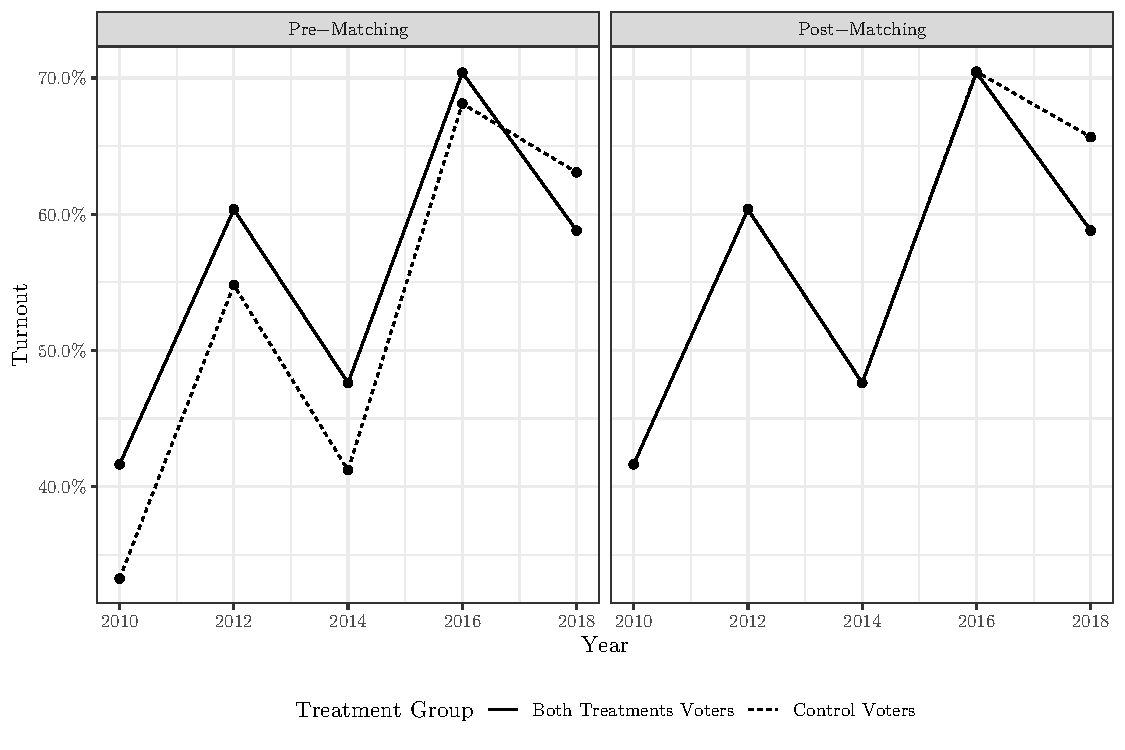
\includegraphics{hurricane_michael_files/figure-latex/full-to-chunk-1} 

}

\caption{\label{fig:full-to}General Election Turnout for Treated and Control Voters, 2010 -- 2018}\label{fig:full-to-chunk}
\end{figure}

Table \ref{tab:full-dind} formalizes Figure \ref{fig:full-to} into a differences-in-differences regression specification. I employ a logistic model, as the dependent variable --- turnout --- is binary. The dependent variable takes the value 1 if a voter cast a ballot in a given year, and 0 if she did not. Model 1 includes only three variables in addition to the constant. \emph{D(Treated)} measures the gap between treated and control voters in the 2010 -- 2016 period. \emph{D(2018)} measures the increase in turnout observed among control voters in 2018, while \emph{D(Treated) × D(2018)} measures whether turnout in 2018 departed further or less from the baseline for the treated voters than the control voters. Model 2 includes the same variables, but also includes the characteristics on which the voters were matched. Model 3, finally, also includes measures for congressional district competitiveness. Because this variable is ``downstream'' of treatment --- that is to say, the effect of the hurricane could have impacted the competitiveness of certain races --- it is not included in the first two models. It should be noted that each of the treated voters lived in uncontested congressional districts. Robust standard errors are clustered at the level of the match (Abadie and Spiess \protect\hyperlink{ref-Abadie2019}{2019}).

\begin{singlespace}

\input{"../temp/dind_full.tex"}
\end{singlespace}

Exponentiating the coefficients in Table \ref{tab:full-dind} indicates that Hurricane Michael, net of any county- and state-level responses, reduced turnout by between 28.3 and 32.3 percentage points.

There was substantial differences in the depressed turnout in the different counties. Turnout in Bay, Calhoun, and Jackson Counties, for instance, was between 60 and 70 percent of what it would have been absent the hurricane; counterintuitively, the treatment effect in Franklin County is associated with a 20 to 23 percentage point increase in turnout. Figure \ref{fig:county-effects} plots the treatment effect for each county.

\begin{figure}[H]

{\centering 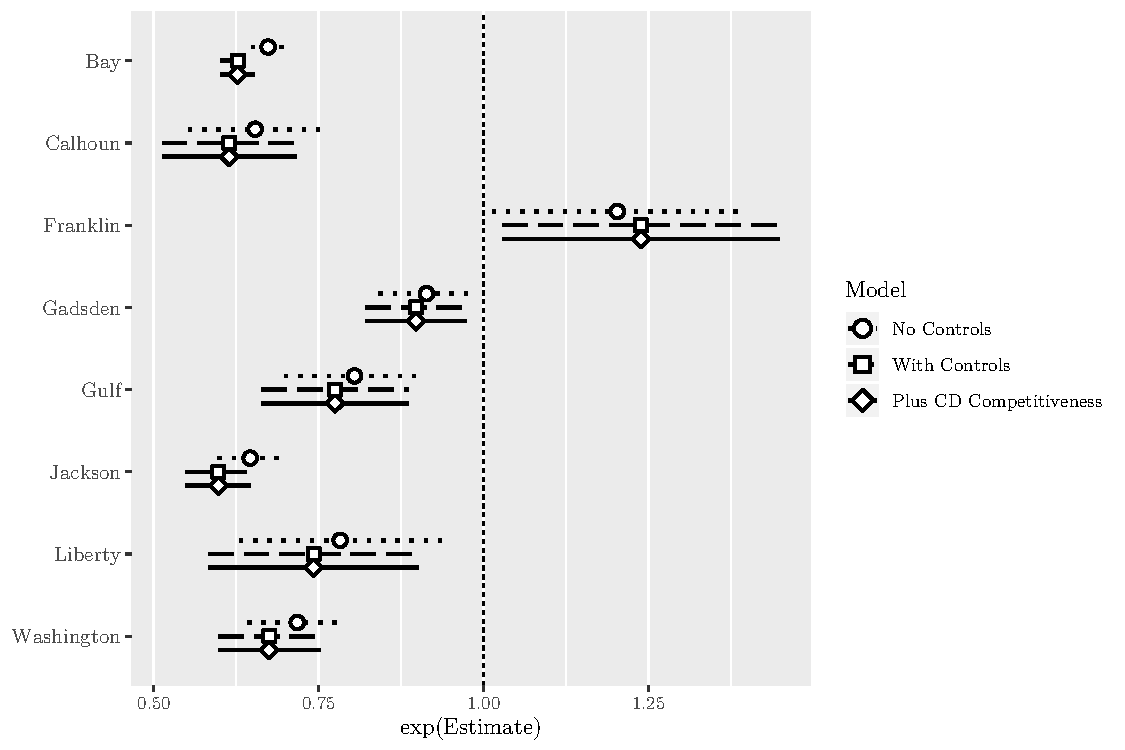
\includegraphics{hurricane_michael_files/figure-latex/county-effect-chunk-1} 

}

\caption{\label{fig:county-effects}Treatment Effect by Treated County}\label{fig:county-effect-chunk}
\end{figure}

\hypertarget{identifying-adminstrative-effects}{%
\subsection*{Identifying Adminstrative Effects}\label{identifying-adminstrative-effects}}
\addcontentsline{toc}{subsection}{Identifying Adminstrative Effects}

As discussed above, our primary strategy for isolating the administrative effects of the hurricane on turnout involves leveraging random assignment around county borders in the Florida panhandle. We begin by identifying all voter precincts in ``treated'' counties that border voter precincts in ``untreated'' counties. Figure \ref{fig:map} shows the border precincts in treated and untreated counties, as well as the precincts that do not fall along the border of a county with a different treatment status. Border precincts in treated counties are in the darkest shade of gray; border precincts in untreated counties are slightly lighter; the precincts that are not used for this analysis are in the lightest shade. Precinct borders are drawn in white, while county borders are drawn in black. Because Gulf and Calhoun Counties are entirely surrounded by other treated counties, no precincts from these counties are used in this analysis.

\begin{figure}[H]

{\centering 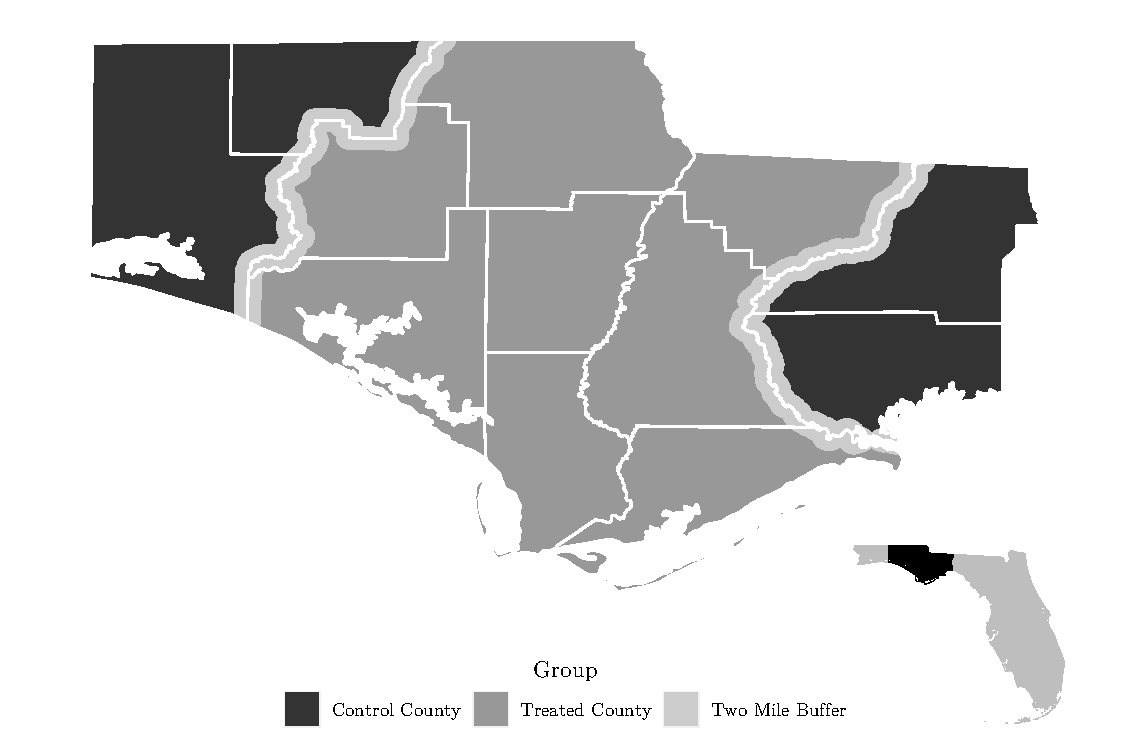
\includegraphics{hurricane_michael_files/figure-latex/map-chunk-1} 

}

\caption{\label{fig:map}Treated, Control, and Discarded Precincts in the Treated Region}\label{fig:map-chunk}
\end{figure}

Each voter in a treated, border precinct is matched with one voter in a neighboring precinct in an untreated county, once again using the genetic matching algorithm developed by Sekhon (\protect\hyperlink{ref-Sekhon2011}{2011}). In some cases, precincts on either side of the border are in different congressional districts. This would pose a problem if these races were contested, but every precinct included was located entirely in an uncontested congressional district.\footnote{One precinct pair, however, is excluded: the Liberty County 5th Precinct was located in a congressional district that went uncontested by Democrats, but borders Precinct 2365 in Leon County, located in a district uncontested by a Republican. All other cross-county precinct pairs faced the same congressional race landscape.} As before, we match on individual- and neighborhood-level characteristics. Table \ref{tab:balance-ll} presents the results of this matching exercise.

\begin{singlespace}
\begin{table}[H]

\caption{\label{tab:balance-tab-ll}\label{tab:balance-ll} Balance Table for Border Precinct Matching}
\centering
\resizebox{\linewidth}{!}{
\begin{tabular}[t]{lllllrrrr}
\toprule
\multicolumn{1}{c}{ } & \multicolumn{2}{c}{Means: Unmatched Data} & \multicolumn{2}{c}{Means: Matched Data} & \multicolumn{4}{c}{Percent Improvement} \\
\cmidrule(l{3pt}r{3pt}){2-3} \cmidrule(l{3pt}r{3pt}){4-5} \cmidrule(l{3pt}r{3pt}){6-9}
 & Treated & Control & Treated & Control & Mean Diff & eQQ Med & eQQ Mean & eQQ Max\\
\midrule
\%White & 75.0\% & 83.0\% & 75.0\% & 75.0\% & 99.91 & 99.93 & 99.93 & 99.93\\
\% Black & 21.0\% & 12.0\% & 21.0\% & 21.0\% & 99.31 & 99.30 & 99.30 & 99.30\\
\% Latino & 2.0\% & 2.0\% & 2.0\% & 2.0\% & 99.88 & 100.00 & 100.00 & 100.00\\
\% Asian & 0.0\% & 1.0\% & 0.0\% & 0.0\% & 93.07 & 93.05 & 93.05 & 93.05\\
\% Female & 53.0\% & 53.0\% & 53.0\% & 53.0\% & 94.65 & 95.16 & 95.16 & 95.16\\
\% Male & 45.0\% & 46.0\% & 45.0\% & 45.0\% & 90.01 & 89.01 & 89.01 & 89.01\\
Age & 52.54 & 51.61 & 52.54 & 52.52 & 98.34 & 67.87 & 60.84 & 43.35\\
\% Democrat & 44.0\% & 39.0\% & 44.0\% & 44.0\% & 99.84 & 99.90 & 99.90 & 99.90\\
\% Republican & 42.0\% & 45.0\% & 42.0\% & 42.0\% & 98.65 & 98.58 & 98.58 & 98.58\\
\% with Some College & 64.0\% & 67.0\% & 64.0\% & 67.0\% & -27.23 & -3.90 & -21.66 & -29.52\\
Median Income & \$47,598 & \$49,407 & \$47,598 & \$50,132 & -40.13 & 20.49 & 8.70 & 1.05\\
\bottomrule
\end{tabular}}
\end{table}
\end{singlespace}

Although the matching exercise does not improve the neighborhood-level characteristics, each of the individual-level characteristics are much improved. The lack of balance on the neighborhood-level characteristics does not appear to cause us to violate the parallel trends assumption; as Figure \ref{fig:ll-to} makes clear, the gap between treated and control voters in the 2010 -- 2016 period remains constant.

\begin{figure}[H]

{\centering 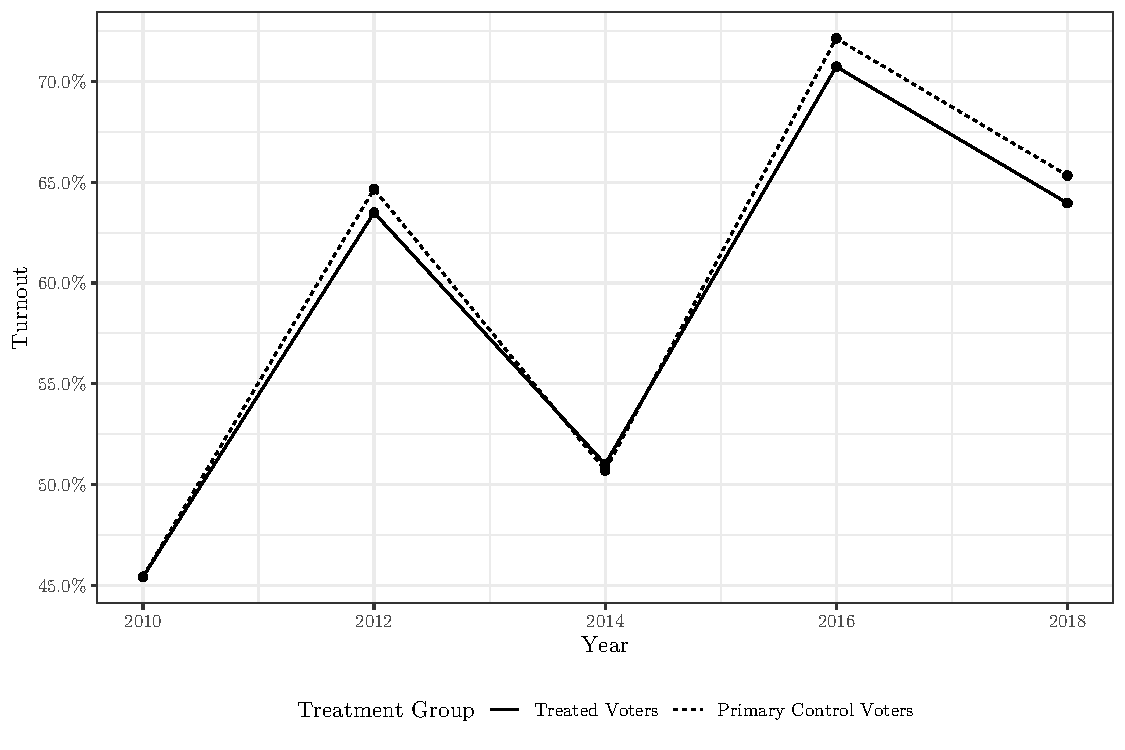
\includegraphics{hurricane_michael_files/figure-latex/ll-to-chunk-1} 

}

\caption{\label{fig:ll-to}General Election Turnout for Border Precinct Matches, 2010 -- 2018}\label{fig:ll-to-chunk}
\end{figure}

The trends in Figure \ref{fig:ll-to} are demonstrate that, even with Executive Order 18-283, there was a substantial, negative administrative effect on turnout: although turnout for voters in the treated group was generally higher in the 2010 -- 2016 period, the difference disappeared in 2018. The control voters, in fact, turned out at higher rates in 2018 than the control voters. Table \ref{tab:dind-ll} formalizes Figure \ref{fig:ll-to} into a logistic regression. Model 1 re-estimates the overall turnout effects presentend in Table \ref{tab:full-dind}, but includes only the voters who live in the border precincts (and, of course, their five matches from elsewhere in the state). This allows us to see the overall effect of the hurricane on these treated voters. Models 2 and 3 estimate the administrative effects of the hurricane on turnout using the treated voters and their matches from bordering precincts. Model 2 includes only the difference-in-differences dummies, while Model 3 adds in the characteristics on which the matching was performed. In all three models, robust standard errors are clustered at the level of the match (Abadie and Spiess \protect\hyperlink{ref-Abadie2019}{2019}).

\begin{singlespace}

\input{"../temp/dind_ll.tex"}
\end{singlespace}

Comparing Model 1 in Table \ref{tab:dind-ll} to Model 3 in Table \ref{full-dind} makes clear that the total effect of the hurricane was much less severe for voters at the very edges of treated counties than for all voters in treated counties: the overall effect for treated voters at the borders was just 16.6 percentage points, compared to 32.3 percentage points for all treated voters. This is unsurprising: voters at the outermost points in the treated counties were probably subjected to much less severe weather than individuals toward the center of the treatment area.

Models 2 and 3 take these same voters and compare their turnout to other voters who we assume faced the same weather, but lived in different electoral administrative environments. Holding the weather constant in this way, these models indicate that the administrative effects of the hurricane caused turnout to decrease by between 13.0 and 14.9 percentage points. At least 78 percent of the observed decrease in turnout among these treated individuals who lived in the border precincts, therefore, were due to administrative effects.

As a final test of the administrative effects of Hurricane Michael on turnout in the treated counties, we construct a difference-in-differences-in-differences, or triple differences, model. In the triple differences specification, each \emph{control} observation from Models 2 and 3 in Table \ref{tab:dind-ll} --- in other words, all matched individuals who live in a border precinct in an untreated county --- is matched with five voters from elsewhere in the state, using the same individual- and neighborhood-level characteristics as the previous matching procedures. We then observe how much turnout decreased for these voters, relative to their matches elsewhere in the state. This assumed to be the depressive effect of weather on turnout, as county election administration in these counties was largely unaffected by the storm. Any observed decrease in turnout among our treated voters above-and-beyond the observered decrease in this control set can then be interpreted as the administrative effect of the storm.

This model is estimated by the following equation:

\(Y_{it}=b_0+b_1D(Panhandle)_{i}+b_2D(2018)_{it}+b_3D(Panhandle)_{i}\times D(2018)_{it} + b_4D(Treated)_{i} + b_5D(Treated)_{i}\times D(2018)_{it}\)

where individual \emph{i}'s turnout in year \emph{t} is a function of the year and their location. In the equation, \emph{b\textsubscript{1}D(Pandhandle)\textsubscript{i}} measures the historical difference between voters in the panhandle (both treated and matched, untreated individuals) and the rest of the state. \emph{b\textsubscript{2}D(2018)\textsubscript{it}} measures the statewide change in turnout in 2018 from the baseline, while \emph{b\textsubscript{3}D(Panhandle)\textsubscript{i} × D(2018)\textsubscript{it}} tests whether turnout changed differently in 2018 in the panhandle than it did elsewhere. \emph{b\textsubscript{3}D(Panhandle)\textsubscript{i} × D(2018)\textsubscript{it}}, therefore, is our estimation of the individual-level, or weather related, effect of the hurricane. \emph{b\textsubscript{4}D(Treated)\textsubscript{i}} measures the historical difference between treated and control observations in the border precincts, and \emph{b\textsubscript{4}D(Treated)\textsubscript{i} × D(2018)\textsubscript{it}} tests whether the change in turnout in 2018 was different for voters living in the treated counties than for their matched controls in the panhandle.

\newpage

\hypertarget{references}{%
\section*{References}\label{references}}
\addcontentsline{toc}{section}{References}

\hypertarget{refs}{}
\begin{cslreferences}
\leavevmode\hypertarget{ref-Abadie2019}{}%
Abadie, Alberto, and Jann Spiess. 2019. ``Robust Post-Matching Inference.'' \emph{Working Paper.}

\leavevmode\hypertarget{ref-Parks2018}{}%
Parks, Miles. 2018. ``After Hurricane Michael, Voting 'Is the Last Thing on Their Minds'.'' \emph{NPR.org}, October 25, 2018. \url{https://www.npr.org/2018/10/25/659819848/after-hurricane-michael-voting-is-the-last-thing-on-their-minds}.

\leavevmode\hypertarget{ref-Sekhon2011}{}%
Sekhon, Jasjeet S. 2011. ``Multivariate and Propensity Score Matching Software with Automated Balance Optimization: The Matching Package for R.'' \emph{Journal of Statistical Software} 42 (1): 1--52. \url{https://doi.org/10.18637/jss.v042.i07}.
\end{cslreferences}

\end{document}
